\documentclass[a4paper, 12pt]{article}
\usepackage[margin=1in]{geometry}
\usepackage[english]{babel}
\usepackage[utf8]{inputenc}
\usepackage{tcolorbox}
\usepackage{listings}
\usepackage{color, soul}
\usepackage{xcolor}
\usepackage{amsmath}
\usepackage{mathtools}
\usepackage{graphicx}
\usepackage{textcomp}
\usepackage{url}
\tcbuselibrary{breakable}

%% MATLAB
\definecolor{codegreen}{rgb}{0,0.6,0}
\definecolor{codegray}{rgb}{0.5,0.5,0.5}
\definecolor{codepurple}{rgb}{0.58,0,0.82}
\definecolor{backcolour}{rgb}{0.95,0.95,0.92}

\lstdefinestyle{mystyle}{
	backgroundcolor = \color{backcolour},
	commentstyle = \color{codegreen},
	keywordstyle = \color{magenta},
	numberstyle = \tiny\color{codegray},
	stringstyle=\color{codepurple},
	basicstyle=\ttfamily\footnotesize,
	breakatwhitespace=false,
	breaklines=true,
	captionpos = b,
	keepspaces = true,
	numbers = left,
	numbersep = 5pt,
	showspaces = false,
	showstringspaces = false,
	showtabs = false,
	tabsize = 2
}

\lstset{style=mystyle}

%%%

\begin{document}
\title{BRI509: Introduction to Brain Signal Processing \\ Assignment No. 3}
\author{\underline{\textbf{CANOY RAYMART JAY}} \\ Student ID \#: \underline{\textbf{2020021376}}}
\date{\today}
\maketitle

\begin{itemize}
\item[(a)]{Draw the Bode diagrams of Do(C4), Mi(E4), Sol(G4) and their chord(C4+E4+G4).}

\begin{tcolorbox}[enforce breakable, pad at break = 1mm, break at=17cm,title={Source Code}]
\lstinputlisting[language=Matlab, upquote=true]{Assignment3_2020021376_CanoyRaymartJay.m}
\end{tcolorbox}
\end{itemize}

\begin{itemize}
\item[(b)]{Bode diagram of C4}
\begin{figure}[h!]
\center{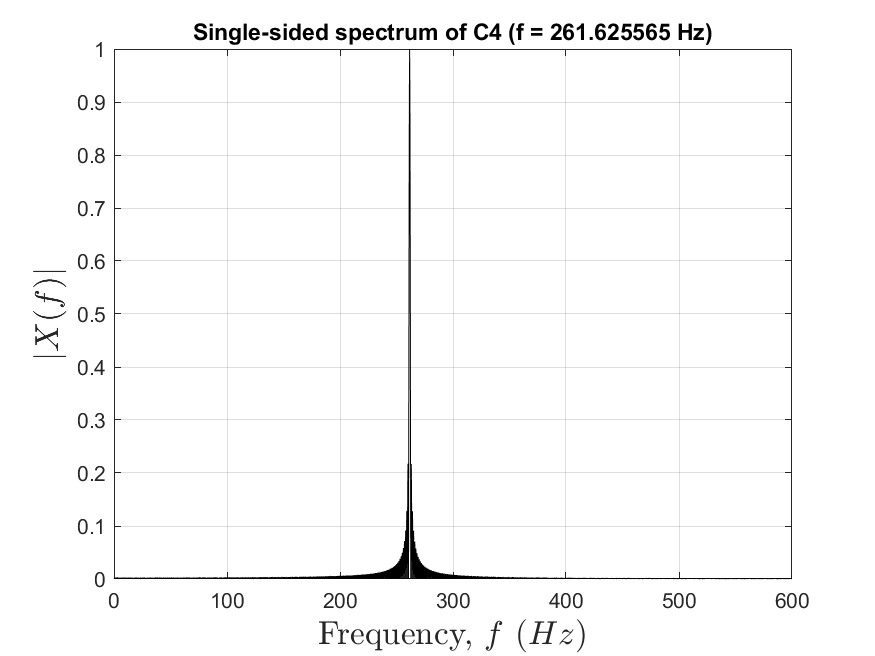
\includegraphics[width=15cm]{FFT_Prob01.png}}
\end{figure}

\pagebreak

\begin{figure}[h!]
\center{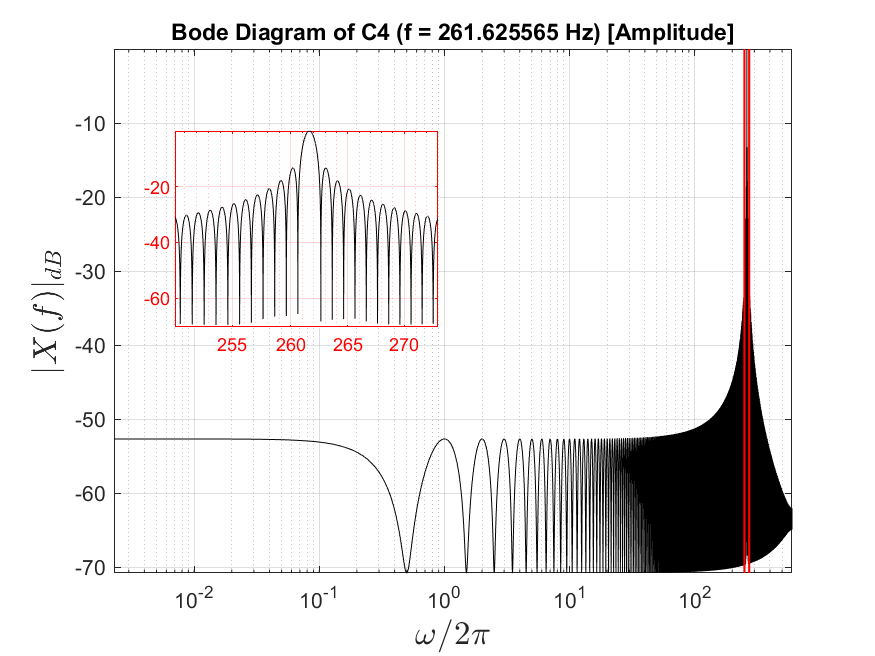
\includegraphics[width=15cm]{Bode_diagram01.png}}
\end{figure}

\begin{figure}[h!]
\center{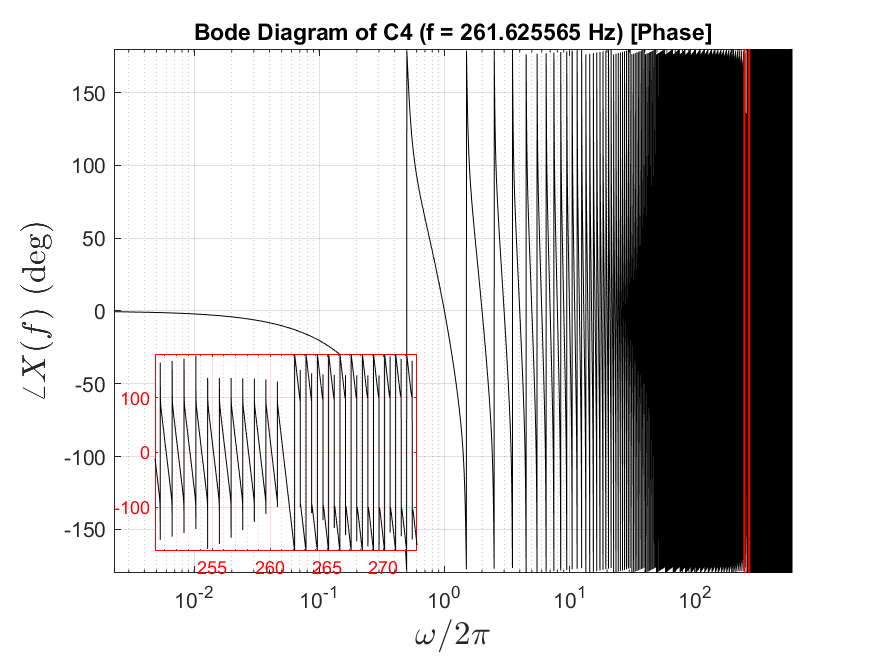
\includegraphics[width=15cm]{Bode_diagram_phase01.png}}
\end{figure}
\end{itemize}

\pagebreak
\begin{itemize}
\item[(c)]{Bode diagram of E4}
\begin{figure}[h!]
\center{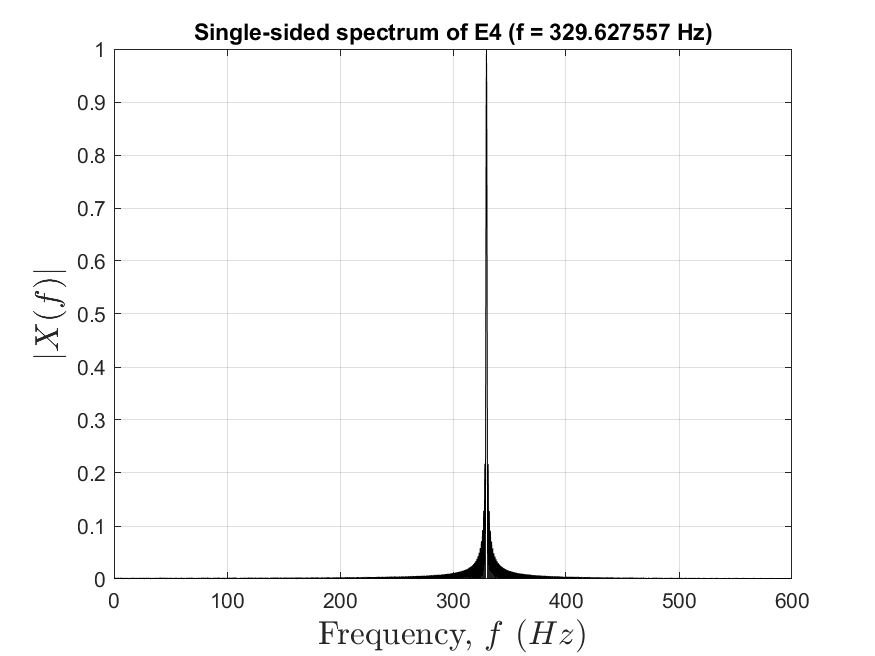
\includegraphics[width=15cm]{FFT_Prob02.png}}
\end{figure}

\begin{figure}[h!]
\center{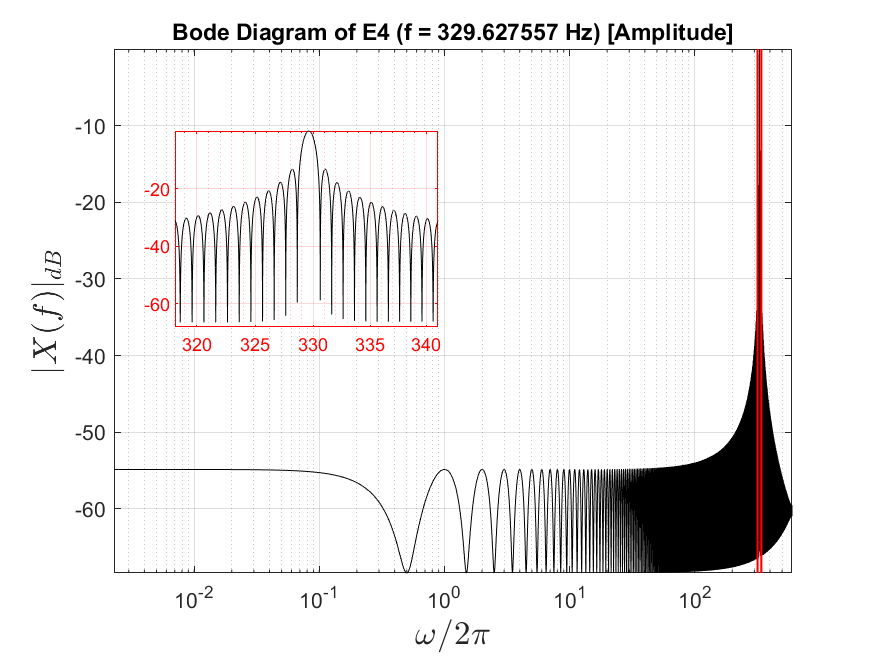
\includegraphics[width=15cm]{Bode_diagram02.png}}
\end{figure}

\pagebreak
\begin{figure}[h!]
\center{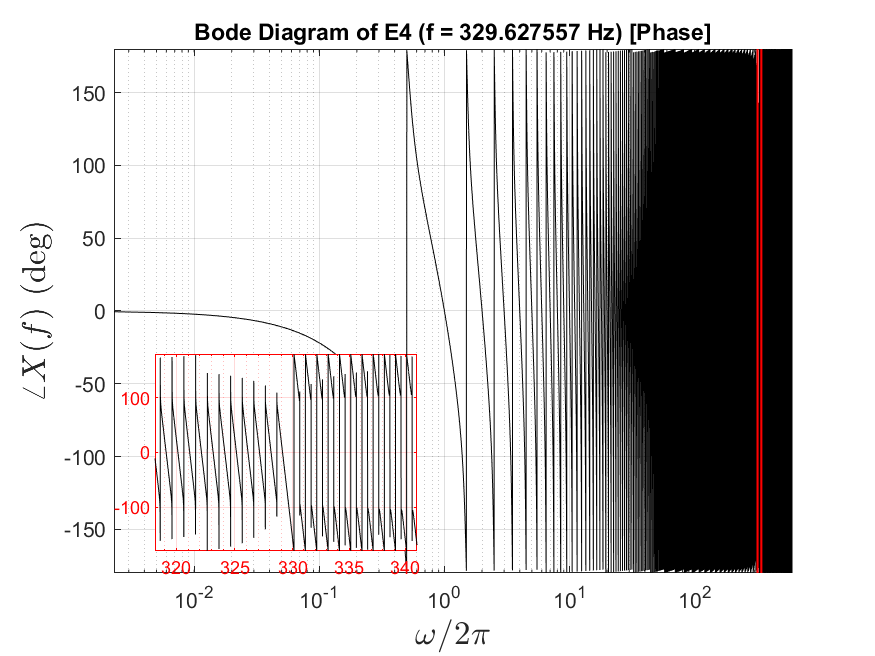
\includegraphics[width=15cm]{Bode_diagram_phase02.png}}
\end{figure}

\item[(d)]{Bode diagram of G4}
\begin{figure}[h!]
\center{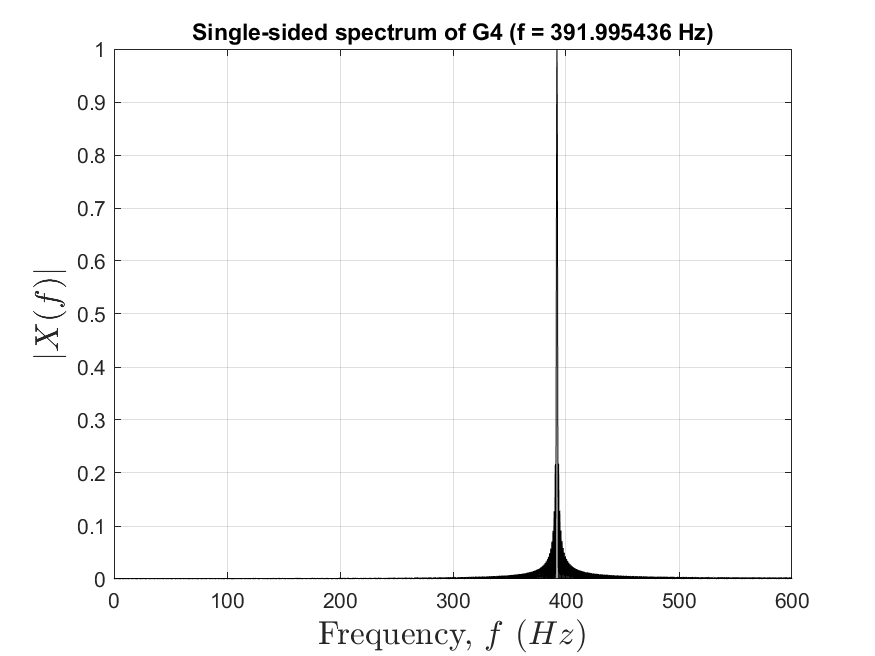
\includegraphics[width=15cm]{FFT_Prob03.png}}
\end{figure}
\pagebreak

\begin{figure}[h!]
\center{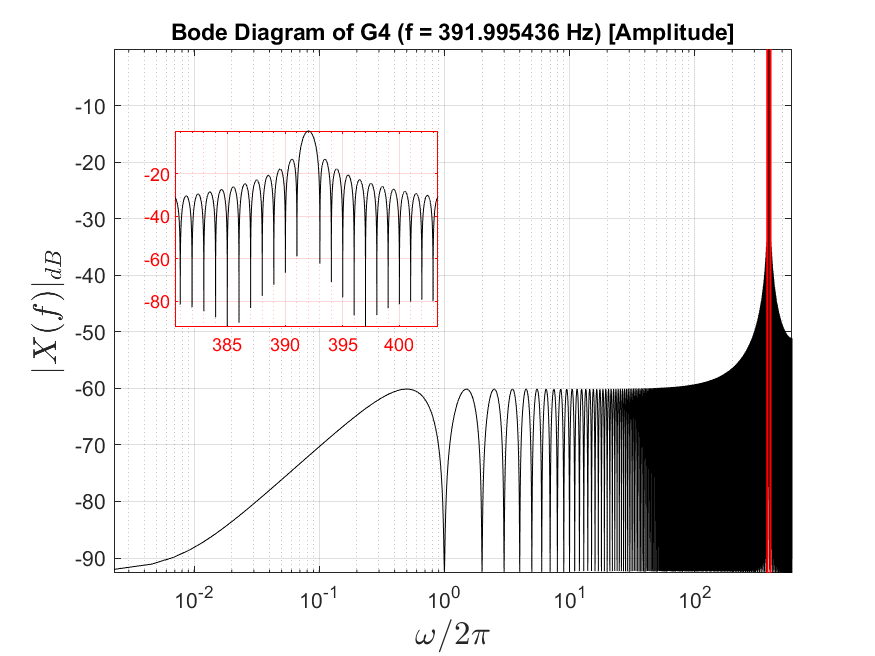
\includegraphics[width=15cm]{Bode_diagram03.png}}
\end{figure}

\begin{figure}[h!]
\center{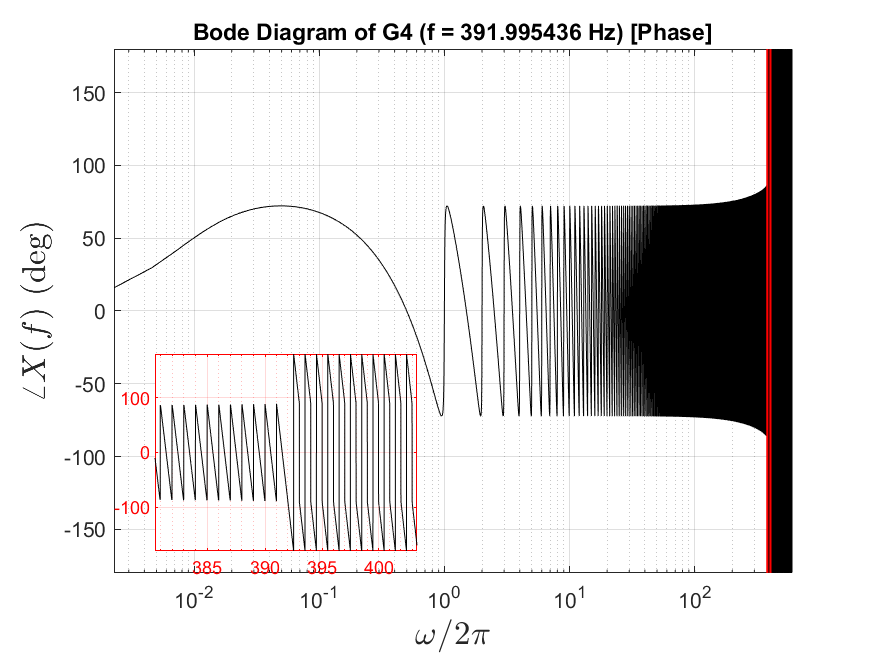
\includegraphics[width=15cm]{Bode_diagram_phase03.png}}
\end{figure}

\pagebreak

\item[(e)]{Bode diagram of C4+E4+G4}

\begin{figure}[h!]
\center{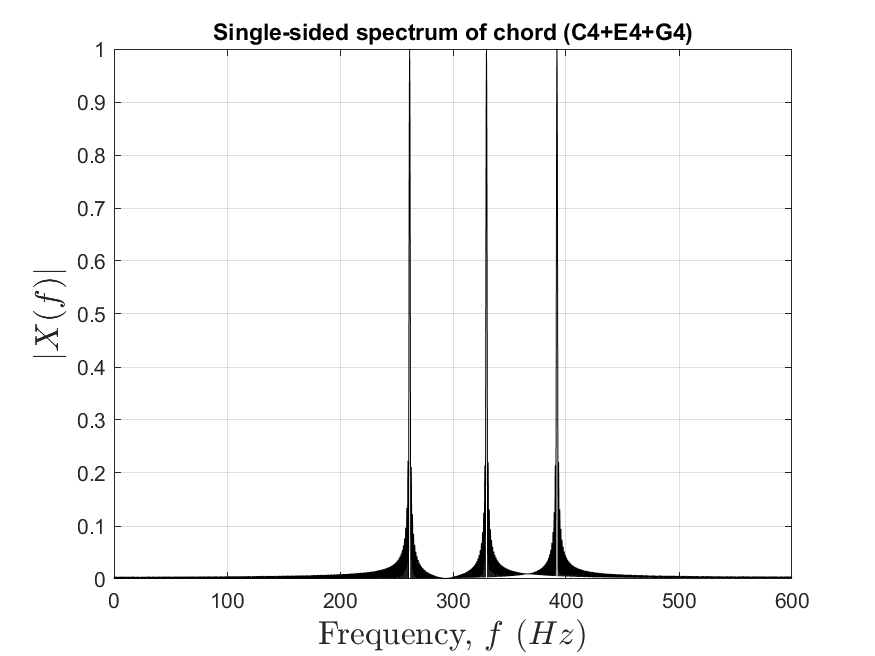
\includegraphics[width=15cm]{FFT_Prob04.png}}
\end{figure}

\begin{figure}[h!]
\center{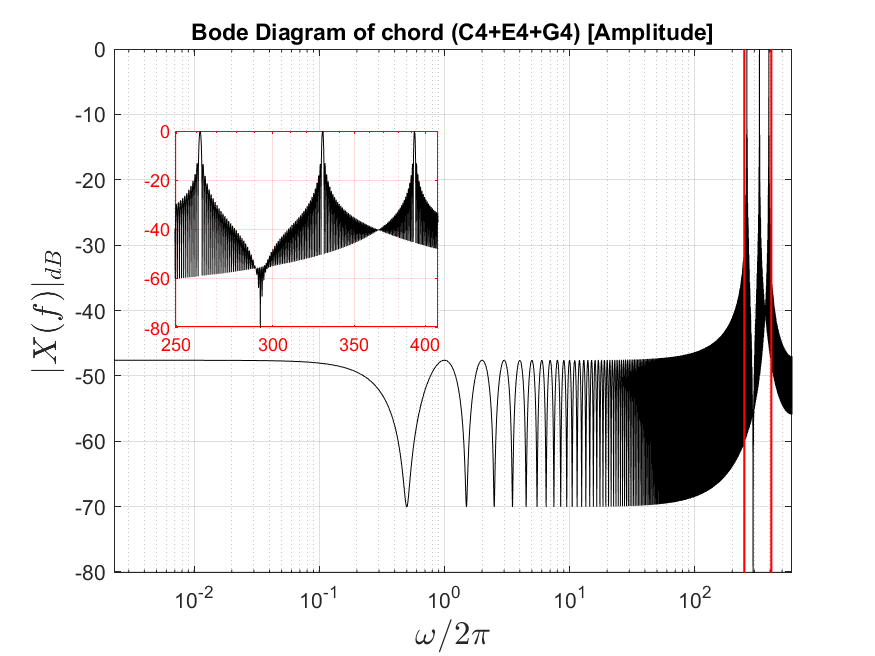
\includegraphics[width=15cm]{Bode_diagram04.png}}
\end{figure}
\pagebreak

\begin{figure}[h!]
\center{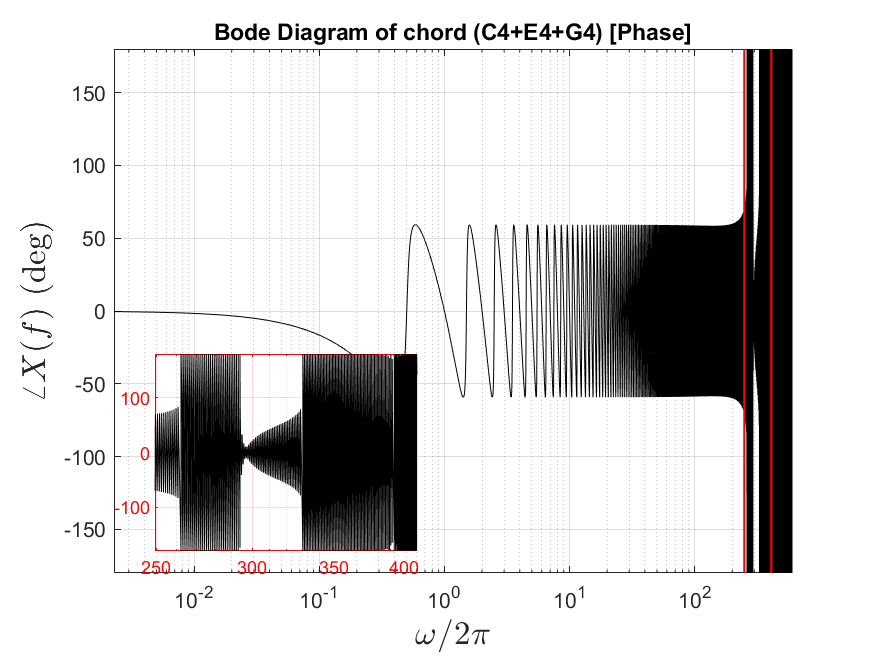
\includegraphics[width=15cm]{Bode_diagram_phase04.png}}
\end{figure}

\vspace{2cm}
\begin{tcolorbox}[title={\textbf{Note: All the files were uploaded on GitHub}}]
All the files in this document were uploaded on Github, and can be accessed at:


\begin{center}
\url{https://github.com/rjcanoy03/BRI509/tree/Assignment%233}
\end{center}


If there are errors in the solution or codes kindly email, $\\$
recanoy@korea.ac.kr.
\end{tcolorbox}
\end{itemize}
\end{document}